\chapter{Process og projektgennemførsel}

I dette afsnittet beskrives gennemførslen af projekten, herunder process, ledelse samt anvendte principper og værktøjer. Disse principper og værktæjer har været et vigtigt elemtent i udarbejdelsen af projektet, og har haft til formål at give arbejet struktur samt at hjælpe grupens til at få et overblik og færdigt og ufærdigt arbejde

\section{SCRUM og agil udvikling}
Scrum er et ”Agile development” værktøj. I dette projekt bruges de væsentligste grunprincipper. Som udgangspunkt er der afholdt et ugentligt ”stå-op” møde, hvor gruppen har talt og diskuteret den forrige uges arbejde, samt hvilke problemer eller forhindringer der har været.

\subsection{Milestones}
En af hoved principperne i scrum er at gøre det der giver mening. Gruppen har derfor ikke brugt scrum "fully dressed" men derimod taget de principper og grundsten med som giver mening på et mindre team.

\subsection{Retrospekt}
Løbende har gruppen revideret samarbejdet i forbindelse med gruppemøder. Dette har givet en stærkere team, og forbedret kommunikationen i mellem gruppens medlemmer.

\subsection{Development spike}
Et princip taget fra "Extreme programming". Dette princip har været brugt i enkelte tilfælde hvor gruppen har arbejdet sig hen mod et mål og ikke stoppet før det nåes.

\section{User Stories}
På tidligere semestre har use cases været brugt til at vise scenarier hvor systemet kan bruges. I dette projekt bruges user stories, som er en kort beskrivelse af en system-feature[ref: http://searchsoftwarequality.techtarget.com/definition/user-story ]. En user story skal forstås som et ønske fra slutbrugerens side, og er altså derved en beskrivelse af et systemkrav.

\subsection{Pivotal Tracker}
Pivotal tracker er et webbaseret, agilt projektsstyrings værktøj, udviklet af pivotal labs[ref:https://www.pivotaltracker.com/]. Pivotal tracker stiller et interaktivt scrumboard til rådighed, hvorpå der er mulighed for at tilføje user-stories til en backlog, tracke teamets velocity samt se opgaver der er færdige. Se eksempel på \ref{fig:scrumboard}.

\begin{figure}
	\centering
	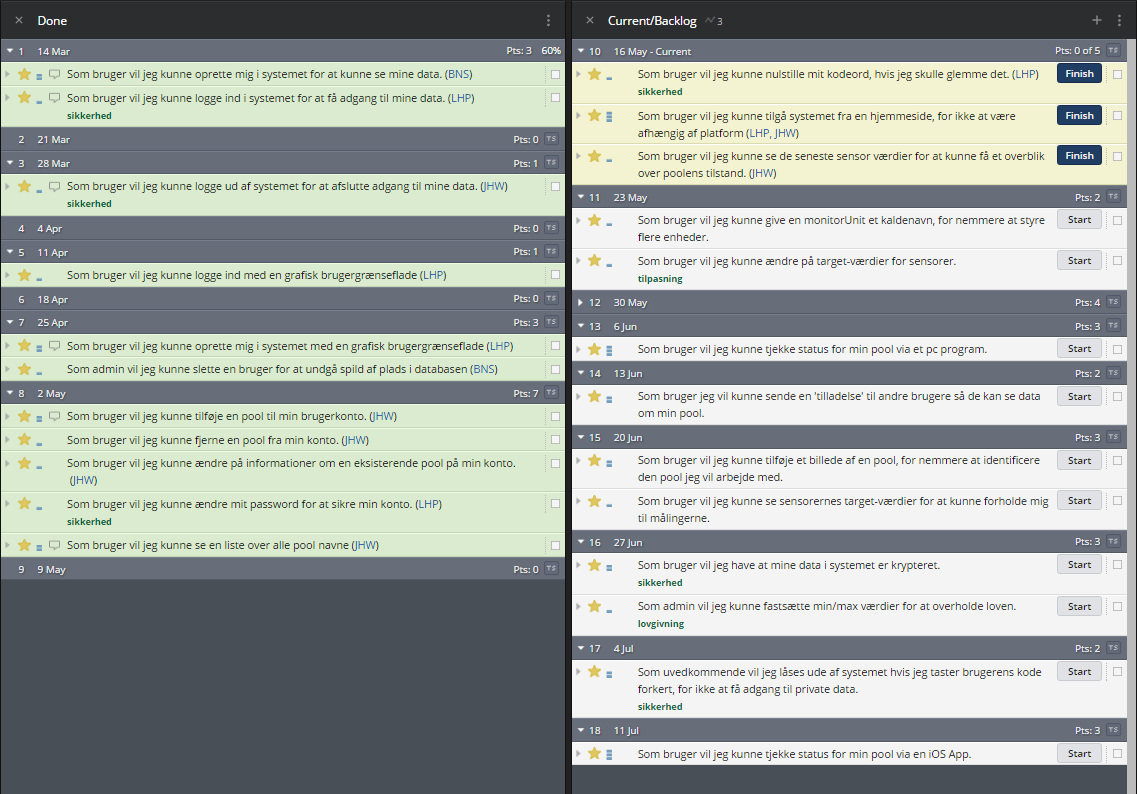
\includegraphics[width=\linewidth]{figs/processProjektGennemforsel/scrumboard.PNG}
	\caption{Pivotal tracker's interaktive scrumboard}
	\label{fig:scrumboard}
\end{figure}

 Da user-stories er meget generelle i forhold til use cases, er der mulighed for at tilføje specificerede tasks til hver user story.

\begin{figure}
\centering
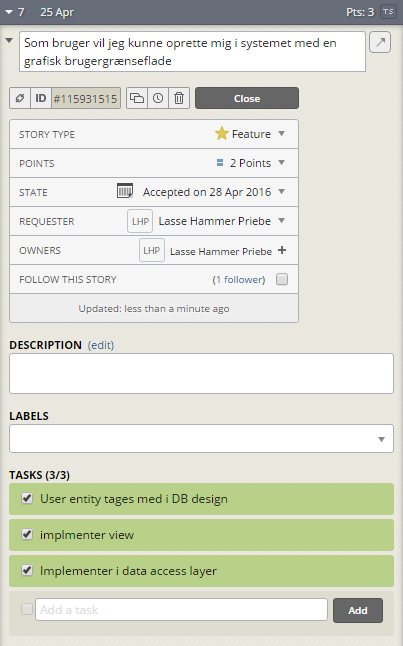
\includegraphics[width=0.5\linewidth]{figs/processProjektGennemforsel/userstory_with_tasks.PNG}
\caption{User Story - Opret Bruger}
\label{fig:userstory_with_tasks}
\end{figure}

Som det ses på \ref{fig:userstory_with_tasks} giver pivotal tracker mulighed for at checke tasks af efterhånden som de udføres. Når der tages hul på en opgave i Pivotal tracker trykkes på knappen start hvorefterden pågældende user story markeres som påbegyndt. Når alle tasks i den pågældende userstory er færdige kan udvikleren trykke på knappen deliver. Skal en anden user så acceptere før den kommer i done? Herefter kan der startes på en ny opgave.

\subsubsection{Estimering}
Når der i fællesskab udarbejdes user stories, bliver teamet samtidig enige og en tidsestimering. I Pvotal Tracker er edr mulighed for at give en user story hhv. 1 2 og 3 point alt efter hvor lang tid, der regnes med at bruge på at udvikle denne feature.  Som det kan ses på \ref{fig:userstory_with_tasks} er der tildelt 3 point til user storyen. Dette er grundet behovet for udvikling af både database, data access, samt GUI. Altså er det en feature der berører alle aspekter af projektet.

\section{Test Driven Development}
TDD er en udviklingsmetode der bla bla bla. Gruppen har brugt TDD i tilfælde hvor bla bla i nogle sprints.

\section{Versionsstyring}
Versionstyring er en vigtig del af softwareudviklingsprocecssen. Det er et værktøj der giver mulighed for at flere udviklere kan arbejde på samme projekt uden at træde hinanden over tæerne.

\subsection{Git}
Gruppen har igennem hele forløbt benyttet versionsstyringsværktøjet Git. Git er gratis, og har været brugt i kurser som Software Test og Indlejret Software Udvikling. Git bruges is projektet til al source kode, og hver feature udikles på sin egen branch. Når en feature er færdig udstedes et pull request, hvorefter repository administratoren kan merge koden ind på master branch. Som en sikkerhedsforanstaltning er Master branchen låst så der ikke uden videre kan pushes til den.

\subsubsection{GitHub}
Github er online hosting af Git repositories, og er brugt i projektet til at gemme source kode, samt administrere projektets repository. I forbindelse med projektstyring og adminitration, har git været brugt til eks. at tracke teamets effektivitet og commit-frekvens.
Projektets repository kan finde på www.github.com/joachimda/I4PRJ.

\subsection{Travis CI og Jenkins}
Gruppen har undervejs forsøgts sig med at arbejde hhv. med Travis CI og Jenkins. Begge værktøjer er til Continuos Integration. CI er er smart idet en ekstern server står for at bygge al source kode der bliver pushet til projektets repository.  Travis CI er gratis til offentlige repositories på GitHub. Dog er Travis CI kun ”community supported” for C\# kode.
Da projektet både indeholder en applikation til PC, iOS, en web applikation, har det været en stor udfordring at benytte et continous integration værktøj.

\section{Software test}
Software testing har været en stor del af dette projekt. Der har været stor fokus på robusthed, og blabla. Der er i alt skrevet XXX automatiserede tests.

\subsection{NUnit og testframeworks}
Et oplagt værktøj til softwaretest har været Nunit idet det bruges i vid udstrækning i forbindelse med kurset Software Test.

\section{UML}
UML er brugt i vid udstrækning gennem alle projektets faser. UML danner grundstenen i projektets dokumentation, men har også hjulpet udviklingen undervejs, idet en visualisering giver bedre forståelse og gør det lettere at gennemskue nye og smartere designmuligheder.

\section{Gruppeledelse og gruppestruktur}